\documentclass[a4paper,11pt]{article}
\usepackage[a4paper]{geometry}
%
%
\usepackage{graphicx}
\usepackage{amssymb,amsmath, amsthm}
\usepackage{mathrsfs}
\usepackage{bbm,bbold}
\usepackage{todonotes}
\usepackage{lineno}
\usepackage{enumitem}

\usepackage{caption}
\usepackage{subcaption}
\usepackage{wrapfig}

%%%%% THEOREM ENVIRONMENTS
\theoremstyle{plain}
\newtheorem{theorem}{Theorem}
\newtheorem{proposition}[theorem]{Proposition}
\newtheorem{lemma}[theorem]{Lemma}
\newtheorem*{lemma*}{Auxiliary Lemma}
\newtheorem{observation}[theorem]{Observation}
\newtheorem{corollary}[theorem]{Corollary}
\newtheorem{fact}[theorem]{Fact}
\newtheorem{conjecture}{Conjecture}
\newtheorem{problem}[theorem]{Problem}
\newtheorem*{conj1}{Conjecture 1}
\newtheorem*{conj2}{Conjecture 2}
\newtheorem*{conj1k2k}{Conjecture 1'}%$_{(k\hookrightarrow 2k)}$}

\theoremstyle{definition}
\newtheorem{definition}[theorem]{Definition}
\newtheorem{remark}[theorem]{Remark}
\newtheorem{remarks}[theorem]{Remarks}
\newtheorem*{acknowledgements}{Acknowledgements}
\newtheorem{example}[theorem]{Example}

\theoremstyle{remark}
\newtheorem{claim}{Claim}

%%% BOLD MATH
\newcommand{\myboldmath}[1]{\mathbbm{#1}}
\newcommand{\R}{\myboldmath{R}}
\newcommand{\G}{\myboldmath{G}}
\newcommand{\Q}{\myboldmath{Q}}
\newcommand{\N}{\myboldmath{N}}
\newcommand{\Z}{\myboldmath{Z}}
\newcommand{\F}{\myboldmath{F}}
\newcommand{\s}{\myboldmath{S}}
\newcommand{\C}{\myboldmath{C}}

\newcommand{\1}{\mathbf{1}}
\newcommand{\E}{\myboldmath{E}}

%%% SIMPLICIAL COMPLEXES AND GRAPHS
\DeclareMathOperator{\st}{st}
\DeclareMathOperator{\lk}{lk}
\newcommand{\bd}{\partial}
\newcommand{\im}{\operatorname{im}}

%%%% OTHER STUFF
\DeclareMathOperator{\supp}{supp}
\newcommand{\up}{\textup{up}}
\newcommand{\down}{\textup{down}} 


\begin{document}
\linenumbers

%%%%OPENING
\title{Hit and Run and Stuff}
\author{Anna Gundert\footnote{Institut f\"{u}r Theoretische Informatik, ETH Z\"{u}rich, CH-8092 Z\"{u}rich, Switzerland. \texttt{anna.gundert@inf.ethz.ch}. Research supported by the Swiss National Science Foundation (SNF Projects 200021-125309 and 200020-138230).} \and May Szedl\'ak\footnote{Institut f\"{u}r Theoretische Informatik, ETH Z\"{u}rich, CH-8092 Z\"{u}rich, Switzerland. \texttt{may.szedlak@inf.ethz.ch}.}}

\begin{titlepage}
\maketitle
\thispagestyle{empty}
%%
The families of solutions for a particular motor task  (i.e., feasible activation sets) are high-dimensional subspaces with a well defined structure that emerges naturally from the interactions among the feasible neural commands, the anatomy of the limb, and the mechanical constraints defining the task.
Characterizing their structure, however, has proven challenging.
Here we present a novel computationally efficient approach to characterize their multi-dimensional structure by uniformly sampling their interior using the Hit-and-Run algorithm---a generalization of a discrete Markov chain.
We studied 3D static force production by a realistic model of the human index finger with 7 muscles and 4 kinematic degrees of freedom.
For each of 9 sub-maximal magnitudes of static fingertip force in a given direction, the feasible activation set is a 4-dimensional convex polytope  embedded in 7-dimensional activation space.
We describe the structure of each feasible activation set by the histograms of feasible activations for individual muscles.  Then, we describe the multi-dimensional interaction among these valid muscle activations and six cost functions using an interactive parallel coordinates system. 
This first description of the multi-dimensional nature of families of feasible solutions  has important consequences to our understanding of the neural control of redundant musculature.  For example, the bounding box of the feasible activation set singularly misconstrues the families of feasible activations—and the modes of the histograms for low magnitudes do not necessarily correspond to those for higher ones. Similarly, exploring and exploiting families of feasible solutions is likely more biologically plausible than searching for unique optimal solutions, and knowing these families will help mitigate biomechanical confounds in dimensionality reduction techniques seeking to extract synergies of neural origin.
More importantly, describing the structure of feasible activation sets as raw or cost-weighted multi-dimensional probability distributions marries neuromechanical and Bayesian perspectives into an integrative probabilistic approach to motor control, dysfunction, rehabilitation, and learning/adaptation for neuromechanically realistic limbs.
%%
\end{titlepage}
%%%%

%%%%ARTICLE
The families of solutions for a particular motor task  (i.e., feasible activation sets) are high-dimensional subspaces with a well defined structure that emerges naturally from the interactions among the feasible neural commands, the anatomy of the limb, and the mechanical constraints defining the task.
Characterizing their structure, however, has proven challenging.
Here we present a novel computationally efficient approach to characterize their multi-dimensional structure by uniformly sampling their interior using the Hit-and-Run algorithm---a generalization of a discrete Markov chain.
We studied 3D static force production by a realistic model of the human index finger with 7 muscles and 4 kinematic degrees of freedom.
For each of 9 sub-maximal magnitudes of static fingertip force in a given direction, the feasible activation set is a 4-dimensional convex polytope  embedded in 7-dimensional activation space.
We describe the structure of each feasible activation set by the histograms of feasible activations for individual muscles.  Then, we describe the multi-dimensional interaction among these valid muscle activations and six cost functions using an interactive parallel coordinates system. 
This first description of the multi-dimensional nature of families of feasible solutions  has important consequences to our understanding of the neural control of redundant musculature.  For example, the bounding box of the feasible activation set singularly misconstrues the families of feasible activations—and the modes of the histograms for low magnitudes do not necessarily correspond to those for higher ones. Similarly, exploring and exploiting families of feasible solutions is likely more biologically plausible than searching for unique optimal solutions, and knowing these families will help mitigate biomechanical confounds in dimensionality reduction techniques seeking to extract synergies of neural origin.
More importantly, describing the structure of feasible activation sets as raw or cost-weighted multi-dimensional probability distributions marries neuromechanical and Bayesian perspectives into an integrative probabilistic approach to motor control, dysfunction, rehabilitation, and learning/adaptation for neuromechanically realistic limbs.
\section{Hit-and-Run}
The Hit-and-Run algorithm used for sampling in a convex body $K$, was introduced by Smith in 1984 \cite{Smith}. The mixing time is known to be $\mathcal{O}^*(n^2R^2/r^2)$, where $R$ and $r$ are the radii of the inscribed and cicumscribed ball of $K$ respectively \cite{Dyer, Lovasz}.
In the case of the muscles of a limb, we are interested in the polygon $P$ that is given by the set of all possible activations $\textbf{a} \in \mathbb{R}^n$ that satisfy
\[\textbf{f} = A\textbf{a}, \textbf{a} \in [0,1]^n,\]
where $\textbf{f} \in \mathbb{R}^m$ is a fixed force vector and $A = J^{-T}RF_m \in \mathbb{R}^{m \times n}$. $P$ is bounded by the unit $n$-cube since all variables $a_i$, $i \in [n]$ are bounded by 0 and 1 from below, above respectively.

Consider the following $1 \times 3$ example.
\begin{align*}
&1 = \frac{10}{3}a_1 - \frac{53}{15}a_2 + 2a_3 \\
&a_1, a_2, a_3 \in [0,1],
\end{align*}
the set of feasible activations is given by the shaded set in figure ??.

\textit{\textbf{FIGURE 1}}

The Hit-and-Run walk on $P$ is defined as follows (it works analogously for any convex body). 
\begin{enumerate}
\item Find a given starting point $\textbf{p}$ of $P$ .
\item Generate a random direction through $\textbf{p}$ (uniformly at random over all directions).
\item Choose the next point of the sampling algorithm uniformly at random from the segment of the line in $P$. 
\item Repeat from $(b)$ the above steps with the new point as the starting point.
\end{enumerate}

\textit{
\textbf{FIGURE 2}: Figures in 2D or 3D? Better in 3D to have the overview.
\begin{enumerate}
\item figure inner point
\item figure choice of direction
\item figure line segment
\item figure choice of new point
\item figure of distribution after some sampling
\end{enumerate}}

The implementation of this algorithm is straight forward except for the choice of the random direction. How do we sample uniformly at random (u.a.r.) from all directions in $P$? Suppose that $\textbf{q}$ is a direction in $P$ and $p \in P$. Then by definition of $P$, $\textbf{q}$ must satisfy $\textbf{f} = A(\textbf{p}+\textbf{q})$. Since $\textbf{p} \in P$, we know that $\textbf{f} = A\textbf{p}$ and therefore 
\[\textbf{f} = A(\textbf{p} + \textbf{q}) = \textbf{f} + A\textbf{q}\]
and hence
\[A\textbf{q} = 0.\]

\textit{\textbf{FIGURE 3}: $q$ must be parallel to the plane given by $1 = \frac{10}{3}a_1 - \frac{53}{15}a_2 + 2a_3$.}

We therefore need to choose directions uniformly at random from all directions in the vectorspace 
\[V = \{\textbf{q} \in \mathbb{R}^n | A\textbf{q} = 0\}.\]

As shown by Marsaglia this can be done as follows \cite{Marsaglia}.

\begin{enumerate}
\item
Find an orthonormal basis $b_1, \dots, b_r \in \mathbb{R}^{n}$ of $A\textbf{q} =0$.
\item
Choose $(\lambda_1, \dots, \lambda_r) \in \mathcal{N}(0,1)^n$ (from the Gaussian distribution).
\item
$\sum_{i=1}^r \lambda_i b_i$ is a u.a.r.\ direction.
\end{enumerate}

A basis of a vectorspace $V$ is a minimal set of vectors that generate $V$, and it is orthonormal if the vectors are pairwise orthogonal (perpendicular) and have unit length. Using basic linear algebra one can find a basis for $V = \{A\textbf{q} = 0\}$ and orthogonalize it with the well known Gram-Schmidt method (for details see e.g.\ \cite{Robertson}). Note that in order to get the desired u.a.r.\ distribution the basis needs to be orthonormal. For the limb case we can safely assume that the rows of $A$ are linearly independent and hence the number of basis vectors is $n-m$.

\textit{\textbf{FIGURE 4}
\begin{enumerate}
\item Some basis
\item orthonormal basis
\end{enumerate}}
%\input{Proof1.tex}
%\input{Proof2.tex}
%\input{concluding.tex}\todo{???}

%%%%
\bibliographystyle{plain}
\bibliography{redundancyFVC}
%\section{APPENDIX}

\subsection{Finger model data}
$F_o = (123.0, 219.0, 23.52, 91.74,	21.6, 124.8, 129.6)$\\
$
JR = 
\begin{pmatrix}
-0.08941 & -0.0447 & -0.009249 & 0.03669 & 0.1421 & 0.2087 & -0.2138 \\
-0.04689 & -0.1496 & 0.052 &0.052 & 0.0248 & 0.0 & 0.0248 \\ 
0.06472 & 0.001953 & -0.1518 &-0.1518 & 0.2919 & 0.0568 & 0.2067 \\
0.003081 & -0.002352 & -0.0001649 & -0.0001649 & -0.0004483 & 0.0001578 & -0.000685
\end{pmatrix}
$
$task_x = (1.0,0.0,0.0,0.0)$
$task_y = (0.0,1.0,0.0,0.0)$
Palmar force is $task_z = (0.0,0.0,1.0,0.0)$
$task_xy = (1.0,1.0,0.0,0.0)$

\begin{figure}[h]
\centering
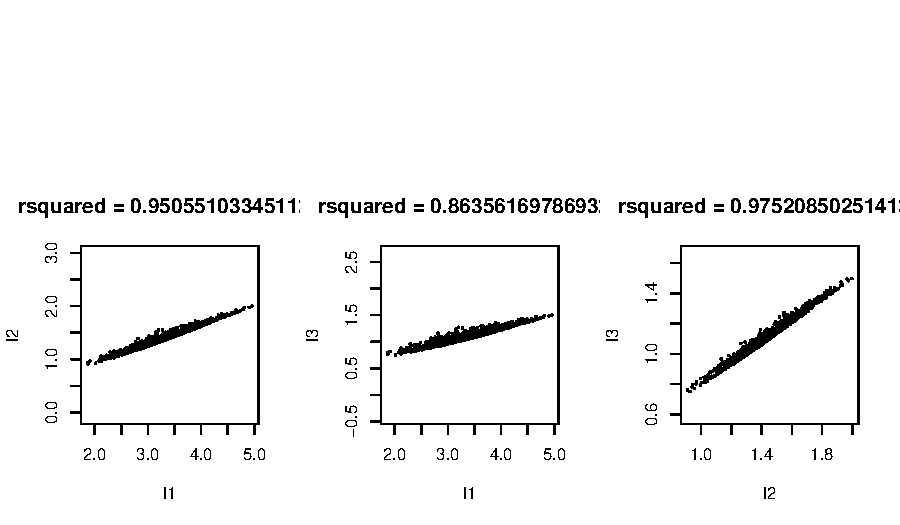
\includegraphics[width=0.5\textwidth,page=1]{figs/cost_function_scatterplots.pdf}
\caption{Nonweighted cost functions}
\label{fig:unweighted_cost_functions}
\end{figure}

\begin{figure}[h]
\centering
\includegraphics[width=0.5\textwidth,page=2]{figs/cost_function_scatterplots.pdf}
\caption{Weighted cost functions}
\label{fig:weighted_cost_functions}
\end{figure}
\end{document}
